\chapter{SWID Generator}

% {{{ Requirements -----------------------------------------------------------%

\section{Requirements}

\subsection{Zweck}

Der SWID Generator soll ein kleines Programm für Linux-Systeme sein, welches aus
den Informationen in Paket Management Systemen SWID Tags generiert.

\subsection{Nichtfunktionale Anforderungen}

\begin{itemize}
		\item Als Implementationsprache wird Python verwendet.
		\item Es sollen möglichst wenig Abhängigkeiten zu Drittkomponenten wie
			Libraries/Frameworks entstehen.
		\item Die Software soll einfach zu installieren sein, beispielsweise durch
			Upload in den Python Package Index ($\rightarrow$ \texttt{pip install
			swid-generator}) oder durch Erstellen von \texttt{.deb}- und
			\texttt{.rpm}-Paketen.
		\item Als Quelle der Paketinformationen sollen Paketmanager wie DPKG und RPM
			verwendet werden.
\end{itemize}

\subsection{Use Cases}

Nachfolgend sind sind die identifizierten Use Cases für die Client Komponenten
des SWID-Generator aufgeführt.

Dabei werden die folgen drei Systemkomponenten berücksichtigt, welche
gegenseitig über die Standardeingabe und -ausgabe kommunizieren.

\vspace{1em}

\begin{figure}[H]
	\centering
	\definecolor{StrongswanColor}{RGB}{199,108,107}
\definecolor{GeneratorColor}{RGB}{116,143,204}
\definecolor{PkgMgrColor}{RGB}{227,225,107}

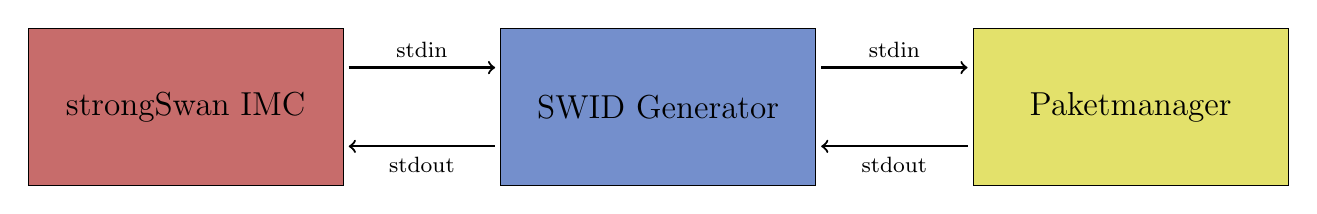
\begin{tikzpicture}[
		actor/.style={font=\large},
		communication/.style={thick, shorten <= 2pt, shorten >= 2pt, font=\footnotesize}
	]

	% Rectangles
	\filldraw[fill=StrongswanColor] (0, 0) rectangle node[actor] {strongSwan IMC} (4, 2);
	\filldraw[fill=GeneratorColor] (6, 0) rectangle node[actor] {SWID Generator} (10, 2);
	\filldraw[fill=PkgMgrColor] (12, 0) rectangle node[actor] {Paketmanager} (16, 2);

	% Arrows
	\draw[->, communication] (4, 1.5) -- node[above] {stdin} (6, 1.5);
	\draw[<-, communication] (4, 0.5) -- node[below] {stdout} (6, 0.5);
	\draw[->, communication] (10, 1.5) -- node[above] {stdin} (12, 1.5);
	\draw[<-, communication] (10, 0.5) -- node[below] {stdout} (12, 0.5);


\end{tikzpicture}

	\caption{SWID Generator: Systemkomponenten}
	\label{img:swid-generator-aktoren}
\end{figure}

\subsubsection{UC01: Erkennung des Paketmanagers}

\begin{usecase}
\hline
\textbf{Akteur} & strongSwan IMC \\
\hline
\textbf{Story} &
Der Akteur weiss nicht welcher Paketmanager auf dem Zielsystem verwendet wird.
Der SWID Generator soll den verwendeten Paketmanager automatisch erkennen. \\
\hline
\textbf{Standard Szenario} &
Der SWID Generator erkennt den System-Paketmanager automatisch. \\
\hline
\textbf{Alternatives Szenario} &
Mittels optionalem Parameter kann der zu verwendende Paketmanager definiert
werden, die automatische Erkennung wird dadurch übersteuert. \\
\hline
\end{usecase}


\subsubsection{UC02: Software ID Generierung}

\begin{usecase}
\hline
\textbf{Akteur} & strongSwan IMC \\
\hline
\textbf{Story} &
Der Akteur will Software IDs aller installierten Pakete generieren. Das Format
dieser IDs folgt dem ISO Draft 19770-2-5 \cite{iso19770-2-5} und besteht
aus der Regid des Tag Creators sowie der Unique ID des Tags. \\
\hline
\textbf{Standard Szenario} &
Alle Software IDs werden generiert und auf der Standardausgabe durch Newlines
(\texttt{\textbackslash{n}}) getrennt ausgegeben. Es wird eine Software ID pro Zeile
ausgegeben. \\
\hline
\textbf{Alternatives Szenario} &
Die Trennzeichen zur Ausgabe der Software IDs können mittels optionalem
Parameter spezifiziert werden. \\
\hline
\end{usecase}


\subsubsection{UC03: SWID Tag Generierung}

\begin{usecase}
\hline
\textbf{Akteur} & strongSwan IMC \\
\hline
\textbf{Story} &
Der Akteur will SWID Tags aller installierten Pakete generieren. Das Format
dieser Dokumente folgt dem ISO Draft 19770-2-5 \cite{iso19770-2-5}. Für jedes
installierte Paket wird ein eigenes XML Dokument generiert. \\
\hline
\textbf{Standard Szenario} &
Alle Tags werden generiert und auf der Standardausgabe durch Newlines
(\texttt{\textbackslash{n}}) getrennt ausgegeben. Es wird ein Tag pro Zeile
ausgegeben. Die Attribute des Tag Creators werden mit vordefinierten
Standardwerten befüllt. Es sind nur die minimal benötigten Elemente und
Attribute enthalten. \\
\hline
\textbf{Alternatives Szenario 1} &
Die Attribute des Tag Creators können mittels optionalen Parametern spezifiziert
werden. \\
\hline
\textbf{Alternatives Szenario 2} &
Die Trennzeichen zur Ausgabe der Tags können mittels optionalem Parameter
spezifiziert werden. \\
\hline
\textbf{Alternatives Szenario 3} &
Zu Debug-Zwecken können die Tags mittels optionalem Parameter in einer
eingerückten und einfacher lesbaren Form ausgegeben werden (\enquote{pretty
printing}). \\
\hline
\textbf{Alternatives Szenario 4} &
Mittels optionalem Parameter können die XML Tags mit einem Payload-Element
versehen werden, welches für jedes Paket die darin enthaltenen Dateien
auflistet. \\
\hline
\end{usecase}


\subsubsection{UC04: Targeted Request}

\begin{usecase}
\hline
\textbf{Akteur} & strongSwan IMC \\
\hline
\textbf{Story} &
Der Akteur möchte nur den SWID Tag eines bestimmten Paketes erhalten. \\
\hline
\textbf{Standard Szenario} &
Mittels Parameter kann dem Generator ein Filterwert angegeben werden,
um einen bestimmten Tag herauszufiltern. Als Filterwert gibt es 2 Varianten:
Entweder über den Package Name oder über die Software ID. \\
\hline
\textbf{Alternatives Szenario 1} &
Die Attribute des Tag Creators können mittels optionalen Parametern spezifiziert
werden. \\
\hline
\textbf{Alternatives Szenario 2} &
Zu Debug-Zwecken können die Tags mittels optionalem Parameter in einer
eingerückten und einfacher lesbaren Form ausgegeben werden (\enquote{pretty
printing}). \\
\hline
\textbf{Alternatives Szenario 3} &
Mittels optionalem Parameter können die XML Tags mit einem Payload-Element
versehen werden, welches für jedes Paket die darin enthaltenen Dateien
auflistet. \\
\hline
\end{usecase}

% }}}

% {{{ Paketmanager -----------------------------------------------------------%

\section{Paketmanager}
\label{swidgenerator:paketmanager}

Im Rahmen dieser Arbeit wurde die Unterstützung für drei der am weitesten
verbreiteten Paketverwaltungssysteme (DPKG, RPM und Pacman) implementiert. Damit
werden 8 der 10 führenden Linux- und BSD-Distributionen gemäss
DistroWatch.com\cite{distrowatch:2014} abgedeckt.

Ein Paketmanager verwaltet unter anderem alle verfügbaren und installierten
Softwarepakete inklusive Meta-Informationen wie Paketname, Version oder
Installationsstatus.

\subsection{DPKG}

DPKG\footnote{\url{https://alioth.debian.org/projects/dpkg}} (Abkürzung für
\textit{Debian Package}) ist die Basis der Paketverwaltung in Debian und in
verwandten Distributionen wie Ubuntu.

\textbf{Liste installierter Pakete abfragen}

\begin{bashcode}
dpkg-query --show --showformat='${Package}\t${Version}\t${Status}\n'
\end{bashcode}

\textbf{Dateien zu Paket abfragen}

\begin{bashcode}
dpkg-query --listfiles <package-name>
\end{bashcode}

\textbf{Bemerkungen}

Entfernte DPKG Pakete können einen sogenannten RC Status haben. Dieser liegt
vor, wenn ein Paket deinstalliert wurde, aber die Konfigurationsdateien auf dem
System belassen wurden. Die \texttt{---show} Option liefert auch diese Pakete.
Der Status ist in der Ausgabe als \texttt{"deinstall ok config-files"}
ersichtlich, entsprechende Pakete können so nachträglich herausgefiltert werden.


\subsection{RPM}

RPM\footnote{\url{https://rpm.org}} (Abkürzung für \textit{Red Hat Package
Manager}) ist der Standard-Paketmanager für Red Hat Linux Systeme sowie
zahlreichen verwandten Distributionen wie openSUSE, Mandriva und Fedora.

\textbf{Liste installierter Pakete abfragen}

\begin{bashcode}
rpm -qa --queryformat %{name}\t%{version}-%{release}
\end{bashcode}

\textbf{Dateien zu Paket abfragen}

\begin{bashcode}
rpm -ql <package-name>
\end{bashcode}


\subsection{Pacman}

Pacman\footnote{\url{https://www.archlinux.org/pacman/}} ist der Paketmanager
unter Arch Linux und allen Derivaten wie Manjaro Linux oder Chakra.

\textbf{Liste installierter Pakete abfragen}

\begin{bashcode}
pacman -Q --color never
\end{bashcode}

\textbf{Dateien zu Paket abfragen}

\begin{bashcode}
pacman -Ql <package-name>
\end{bashcode}

% }}}

% {{{ Architektur ------------------------------------------------------------%

\section{Architektur}

\subsection{Übersicht}

Der SWID Generator wurde komplett in Python geschrieben und nutzt keine externen
Libraries. Es wird sowohl Python 2 wie auch Python 3 unterstützt.

Der Quellcode ist modular aufgebaut, gewisse Komponenten wurden in separate
Subpackages aufgeteilt:

\begin{figure}[H]
	\centering
	\definecolor{GeneratorColor}{RGB}{116,143,204}
\definecolor{GeneratorColorLight}{RGB}{195,206,230}

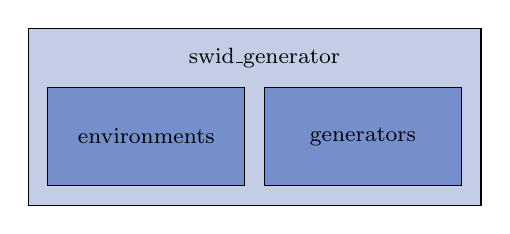
\begin{tikzpicture}[
		package/.style={fill=GeneratorColorLight},
		subpackage/.style={fill=GeneratorColor},
		every node/.style={font=\footnotesize}
	]

	% Packages
	\filldraw[package] (0, 0) rectangle  (5.75, 2.25);

	% Subackages
	\filldraw[subpackage] (0.25, 0.25) rectangle node {environments} (2.75, 1.5);
	\filldraw[subpackage] (3, 0.25) rectangle node {generators} (5.5, 1.5);

	% Labels
	\draw (3, 1.875) node {swid\_generator};

\end{tikzpicture}

	\caption{Aufteilung SWID Generator in Python Packages}
\end{figure}

Das Hauptpackage -- \texttt{swid\_generator} -- enthält folgende Module:

\begin{itemize}
	\item \texttt{main.py}: Der Einstiegspunkt in das Programm
	\item \texttt{argparser.py}: Klassen und Funktionen um
		Kommandozeilenargumente zu parsen
	\item \texttt{print\_functions.py}: Funktionen um Tag- und
		Software-ID-Generatoren auf die Standardausgabe auszugeben
	\item \texttt{package\_info.py}: DTO\footnote{Data Transfer Object, eine
		Klasse die kein Eigenverhalten aufweist sondern lediglich Daten in
		einem Objekt bündelt.}-Klassen für Dateien und Softwarepakete
	\item \texttt{exceptions.py}: Eigene Fehlerklassen
	\item \texttt{settings.py}: Globale Variablen, wie z.\ B.
		\texttt{DEFAULT\_ENTITY\_NAME}
	\item \texttt{meta.py}: Metainformationen zum Generator, wie z.\ B. der
		Programmname, die Lizenz oder die Version
\end{itemize}

Die zwei Subpackages sind für Input respektive Output zuständig. Im
\texttt{environments} Package sind die Environment-Klassen für die verschiedenen
Paketmanager enthalten. Die Klassen greifen auf die jeweiligen Paketdatenbanken
zu und geben diese Informationen an das Hauptprogramm zurück. Auch die
Environment-Registry befindet sich in diesem Package. Mehr dazu im Abschnitt
\ref{swidgenerator:architektur:environments}.

Das \texttt{generators} Package enthält die nötigen Funktionen um aus den (vom
entsprechenden Environment zurückgegebenen) Paketinformationen die dazugehörigen
Software-ID Strings oder SWID XML Tags zu generieren. Diese Funktionen sind als
Python
Generators\footnote{\url{https://docs.python.org/2/tutorial/classes.html\#generators}}
implementiert, die einzelnen Einträge können also schon während der Generierung
laufend ausgegeben werden. Mehr dazu im Abschnitt
\ref{swidgenerator:architektur:printers}.

Als Einstiegspunkt in den SWID Generator dient das \texttt{main.py} Modul. Um
das Programm direkt aus dem Quellcode-Ordner heraus zu starten, sollte Python
mit der \texttt{-m} Option und dem vollständigen Modulpfad gestartet werden:

\begin{bashcode}
python -m swid_generator.main
\end{bashcode}

Wenn das Programm über pip oder setup.py installiert wird (siehe
\autoref{swidgenerator:architektur:deployment}), kann es natürlich auch direkt
über den Programmnamen aufgerufen werden:

\begin{bashcode}
swid_generator
\end{bashcode}

\subsection{Ablauf: Initialisierung}
\label{swidgenerator:architektur:initialisierung}

Wenn der SWID Generator gestartet wird, beginnt die Code-Ausführung im
\texttt{main.py} Modul. Zuerst müssen alle Kommandozeilen-Argumente verarbeitet
werden. Danach müssen die modular aufgebauten Environment Klassen registriert
werden. Mit diesen Informationen muss entschieden werden, welches Environment
dass effektiv verwendet werden soll -- entweder durch den Benutzer definiert
oder durch eine automatische Packetmanager-Erkennung.

Der Ablauf ist wie folgt:

\begin{enumerate}
	\item Die Environment Registry
		(\ref{swidgenerator:architektur:environments:registry}) wird initialisiert.
	\item Alle verfügbaren Environment Klassen
		(\ref{swidgenerator:architektur:environments:interface}) werden der Registry
		übergeben.
	\item Der Argument Parser wird mit einer Referenz auf die Registry instanziert.
	\item Die Parser Instanz parst mithilfe des \texttt{argparse} Moduls aus der
		Python Stanardbibliothek die Kommandozeilen-Argument und generiert daraus ein
		\enquote{Options}-Objekt. \item Dieses Objekt wird nun der Environment Registry
		übergeben. Diese kann mit den Informationen darin die geeignete Environment
		Klasse finden und an das Hauptprogramm zurückgeben. Das Environment kann per
		Kommandozeilen-Argument vorgegeben werden, andernfalls wird es automatisch
		detektiert.
\end{enumerate}

In der folgenden Abbildung ist dieser Ablauf als UML Sequenzdiagramm
dargestellt:

\begin{figure}[H]
	\centering
	\begin{tikzpicture}
	\begin{umlseqdiag}[font=\footnotesize]

		% Objekte

		\umlobject{main}
		\umlcreatecall[dt=5, x=8, class=EnvironmentRegistry]{main}{registry}

		% Calls

		\begin{umlfragment}[type=loop, label=foreach env, inner xsep=10]
			\begin{umlcall}[dt=7, padding=2, op={register(env)}]{main}{registry}
			\end{umlcall}
		\end{umlfragment}

		\umlcreatecall[dt=7, x=4, class=MainArgumentParser]{main}{parser}
		\begin{umlcall}[dt=3, padding=4, op={parse(registry)},return=options]{main}{parser}
		\end{umlcall}

		\begin{umlcall}[dt=7, padding=3, op={get\_environment(options)},return=env]{main}{registry}
			\begin{umlfragment}[type=opt, label=if !options.env, inner xsep=15]
				\begin{umlcallself}[op=autodetect\_env()]{registry}
				\end{umlcallself}
			\end{umlfragment}
		\end{umlcall}

	\end{umlseqdiag}
\end{tikzpicture}

	\caption{Sequenzdiagramm: Initialisierung}
\end{figure}

\subsection{Ablauf: Generierung}
\label{swidgenerator:architektur:generierung}

Nachdem nun im Abschnitt \ref{swidgenerator:architektur:initialisierung} alle
nötigen Informationen gesammelt wurden, kann nun die Hauptarbeit geschehen: Die
Generierung der Daten aus den Paketmanager-Informationen. Ob SWID Tags oder
Software-IDs generiert werden, ist abhängig vom ersten Kommandozeilenargument,
welches entweder \texttt{swid} oder \texttt{software-id} sein kann.

\begin{enumerate}
	\item Zuerst werden mithilfe des SWID Tag Generators
		(\ref{swidgenerator:architektur:generatoren}) die gewünschen Tags aus
		der Paketmanager-Datenbank geholt.
	\item Die zurückgegebenen Tags werden mithilfe der entsprechenden
		Print-Funktionen (\ref{swidgenerator:architektur:printers}) auf die
		Standardausgabe ausgegeben.
	\item Falls im ganzen Programmablauf keine Fehler aufgetreten sind, wird
		das Programm nun mit dem Status Code 0 (=keine Fehler) beendet.
\end{enumerate}

Dieser Ablauf ist im folgenden UML Sequenzdiagramm visualisiert:

\begin{figure}[H]
	\centering
	\begin{tikzpicture}
	\begin{umlseqdiag}

		% Objekte

		\umlobject[x=0]{main}
		\umlobject[x=4]{generator}
		\umlobject[x=6.5]{printer}
		\umlobject[x=9]{sys}

		% Calls

		\begin{umlfragment}[type=alt, label={command = "{}swid"}, inner xsep=23, inner ysep=2]

			\begin{umlcall}[padding=4, dt=10, op=create\_swid\_tags(), return=tags]{main}{generator}
			\end{umlcall}
			\begin{umlcall}[dt=6, op=print\_swid\_tags(tags), return={\ }]{main}{printer}
			\end{umlcall}

			\umlfpart[command = "{}software-id"]

			\begin{umlcall}[padding=4, op=create\_software\_ids(), return=ids]{main}{generator}
			\end{umlcall}
			\begin{umlcall}[dt=0, op=print\_software\_ids(ids), return={\ }]{main}{printer}
			\end{umlcall}

		\end{umlfragment}

		\begin{umlcall}[dt=2, op=exit(0)]{main}{sys}
		\end{umlcall}

	\end{umlseqdiag}
\end{tikzpicture}

	\caption{Sequenzdiagramm: Generierung}
\end{figure}


\subsection{Implementationsdetails: Environments}
\label{swidgenerator:architektur:environments}

Die Environments sind das Kernstück des SWID-Generators, denn sie greifen auf
den System-Paketmanager zu und bereiten die Liste der installierten Pakete für
die weitere Verarbeitung auf.

Wie bereits im Abschnitt \ref{swidgenerator:paketmanager} erwähnt, bietet der
SWID Generator zum aktuellen Zeitpunkt Unterstützung für drei weit verbreitete
Paketmanager an. Damit das Tool in Zukunft auch auf bisher noch nicht
unterstützten Systemen wie Slackware Linux oder FreeBSD einsatzfähig ist, haben
wir grossen Wert darauf gelegt, dass es möglichst einfach ist neue
Environment-Klassen hinzuzufügen und diese zentral zu registrieren.

\subsubsection{Environment Interface}
\label{swidgenerator:architektur:environments:interface}

Um dieses Ziel zu erreichen, ist ein einheitliches Interface für die
Environment-Klassen essentiell.

WIP

\subsubsection{Die Registry}
\label{swidgenerator:architektur:environments:registry}

\subsection{Implementationsdetails: Generatoren}
\label{swidgenerator:architektur:generatoren}

\subsection{Implementationsdetails: Printers}
\label{swidgenerator:architektur:printers}


\subsection{Implementationsdetails: Python 3 Kompatibilität}


\subsection{Packaging}

- Setup.py
- Manifest.in
- meta.py

% }}}

% {{{ Ergebnisse -------------------------------------------------------------%

\section{Ergebnisse}

- Beispiel
- Speed

% }}}

% {{{ Qualitätsmanagement ----------------------------------------------------%

\section{Qualitätsmanagement}
\label{swidgenerator:architektur:qa}

% }}}

% {{{ Deployment -------------------------------------------------------------%

\section{Deployment}
\label{swidgenerator:architektur:deployment}

% }}}
